\documentclass[crop, tikz]{standalone}
\usepackage{tikz}
\usepackage{pgfplots}
\usepackage{xcolor}

% \tikzstyle{invisNode}=[circle, line width=0mm, inner sep=0pt]
% \tikzstyle{smallnode}=[draw, circle, inner sep=2pt]
% \tikzstyle{blackSquareNode}=[draw,minimum size=50pt, minimum height=50pt, inner sep=1pt, fill=black, text=white]
% \tikzstyle{whiteSquareNode}=[draw,minimum size=50pt, minimum height=50pt, inner sep=1pt]
% \tikzstyle{stateTransition}=[-stealth, thick]
% \tikzstyle{line}=[]


\usetikzlibrary{shapes.geometric}
\usetikzlibrary{arrows.meta}

\tikzstyle{stateTransition}=[->, thick, -{Latex[length=2mm,width=2mm]}]

\begin{document}

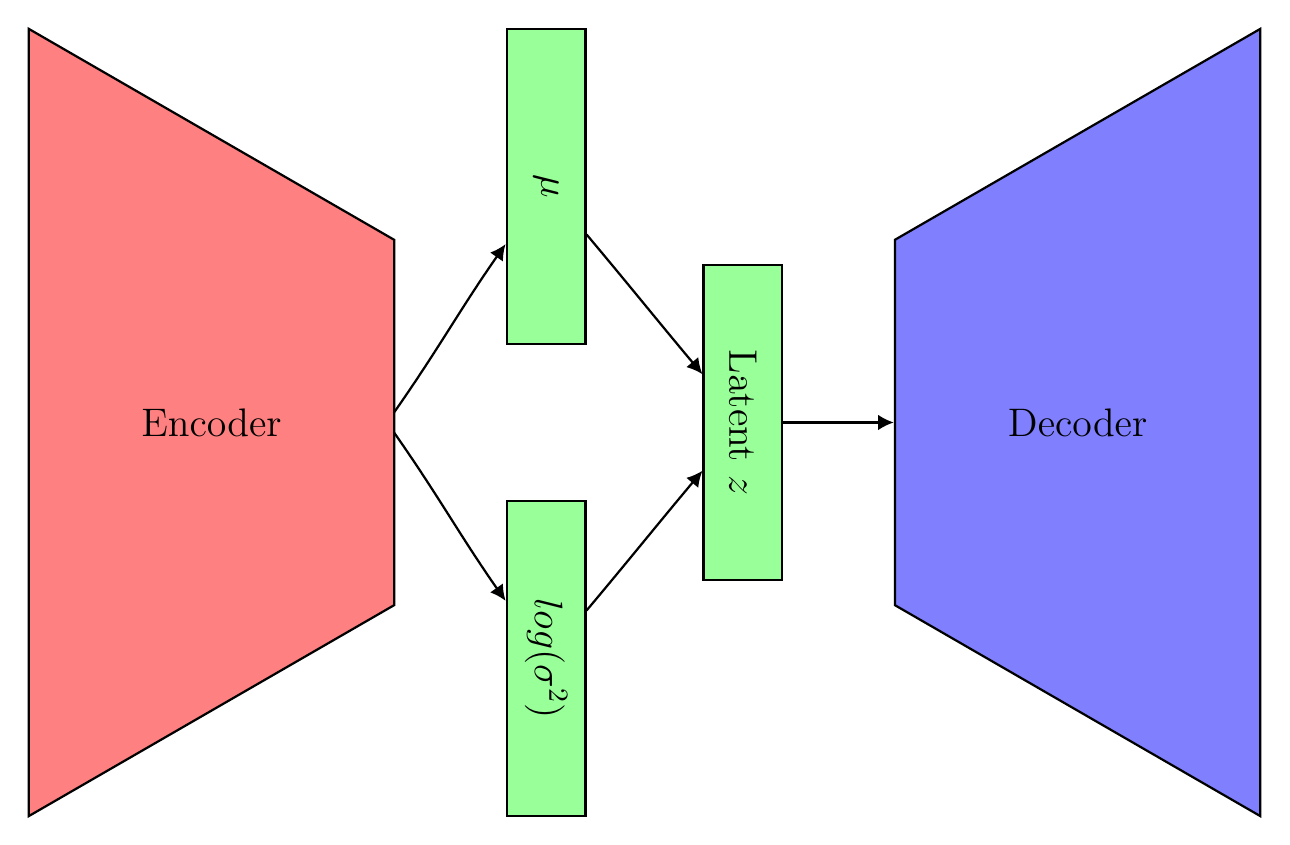
\begin{tikzpicture}
  % Nodes {rgb:red,4;green,2;yellow,1}
  \node [trapezium, fill=red!50, trapezium angle=60, minimum width=10cm, draw, thick, rotate=-90] (encoder) at (-6, 0) {};
   \node (encodertext) at (-6,0) [] {\Large{Encoder}};
   \node (encoderout) at (-3.77,0) [] {};

  \node (mean) at (-1.75,3) [draw, fill=green!40, thick, minimum width=1cm, minimum height=4cm] {};
  \node (meantext) at (-1.75,3) [rotate=-90] {\Large{$\mu$}};

  \node (logvar) at (-1.75,-3) [draw, fill=green!40, thick, minimum width=1cm, minimum height=4cm] {};
  \node (logvartext) at (-1.75,-3) [rotate=-90] {\Large{$log(\sigma^2$)}};

  \node (latent) at (0.75,0) [draw, fill=green!40, thick, minimum width=1cm, minimum height=4cm] {};
  \node (latenttext) at (0.75,0) [rotate=-90] {\Large{Latent $z$}};

  
  \node [trapezium, fill=blue!50, trapezium angle=60, minimum width=10cm, draw, thick, shape border rotate=90] (decoder) at (5, 0){};
  \node (decodertext) at (5,0) [] {\Large{Decoder}};

  % State Transitions
  \draw[stateTransition] (encoderout) to[out=55,in=235] node [midway, sloped, above] {} (mean);
  \draw[stateTransition] (encoderout) to[out=-55,in=-235] node [midway, sloped, above] {} (logvar);
  \draw[stateTransition] (mean) to[out=-50,in=-230] node [midway, sloped, above] {} (latent);
  \draw[stateTransition] (logvar) to[out=50,in=230] node [midway, sloped, above] {} (latent);
  \draw[stateTransition] (latent) to[out=0,in=180] node [midway, sloped, above] {} (decoder);

\end{tikzpicture}

\end{document}